\section{Interference between channels}\label{sec:17.4}

A dark photon that deposits \SI{1.2}{eV} at $q = \SI{1}{keV}$ in silicon can leave an electron--hole pair and a transverse acoustic phonon behind in two ways. It can push the electrons, which then emit the phonon through the electron--phonon coupling: the phonon-assisted amplitude of \cref{sec:13.2}. Or it can push a nucleus, whose electrons lag behind and are excited while the nucleus sheds the phonon: the Migdal amplitude of \cref{sec:12.1}. Both end in the same state, and the rate contains their product as well as their squares. Such products of an electron and a nuclear amplitude fill the bottom row of \cref{tab:8-sectors}, the cross response $S_{e\kappa}$ in each of the three sectors. In the electron-following sector the product cancels the phonon rate of a dark photon in silicon completely. In the two electronic sectors, at small momentum transfer, it raises the rate by 5.5 parts in $10^4$.

\subsection{The three cross cells}\label{sec:17.4-cells}

A mediator that couples to the electrons with the potential $\tilde V_e(\vect{q})$ and to the nuclei of species $\kappa$ with $\tilde V_\kappa(\vect{q})$ has the cross elements $\mathfrak{D}_{e\kappa} = \tilde V_e^*\tilde V_\kappa$ of \cref{eq:8.1-D}, and the rate \cref{eq:8.2-spectrum} contains, besides the electron and the nuclear terms, $2\Real\sum_\kappa\mathfrak{D}_{e\kappa}S_{e\kappa}$. A dark photon couples to $-\tilde Vn_Z$ (\cref{we:8-darkphoton}), so that $\tilde V_e = \tilde V$ and $\tilde V_\kappa = -Z_\kappa\tilde V$. A coupling to electrons alone has $\tilde V_\kappa = 0$, and a coupling to nucleons alone has $\tilde V_e = 0$. For these two the cross response never enters the rate, although $S_{e\kappa}$ itself is not zero, which is why \cref{sec:17.1} could compare the channels cell by cell. For a dark photon the three cells of $S_{e\kappa}$ differ in size by more than three orders of magnitude.

\emph{Electron-following cell.} In this sector the electron density acts on the nuclei as $\bar\rho_e(\vect{q};u)$ of \cref{eq:8.6-follow}. At long wavelength the electrons that follow nucleus $\kappa$ carry the charge $F^{\mathrm{fol}}_\kappa = \hat{\vect{q}}\cdot(Z_\kappa\mathbf{1} - Z^*_\kappa)\cdot\hat{\vect{q}}$, the $q \to 0$ value of $F_{\mathrm{cr}}$ in \cref{eq:12.5-cross}. A phonon then sees the nucleus and its cloud with amplitudes in the ratio $Z_\kappa : F^{\mathrm{fol}}_\kappa$, of opposite sign for a dark photon, and the nuclear, electron and cross terms of its rate stand in the ratio $Z_\kappa^2 : (F^{\mathrm{fol}}_\kappa)^2 : -2Z_\kappa F^{\mathrm{fol}}_\kappa$, which add up to $Z_\kappa^{*2}$. In silicon $F^{\mathrm{fol}} = Z = 14$, and the cross term, $-392$ against $196 + 196$, cancels the other two exactly: a dark photon makes no phonon in silicon at long wavelength (\cref{sec:10.2}). In a polar crystal the cross term removes all but $Z^{*2}$, which $\varepsilon_\infty$ screens further, and what survives is the optical-phonon rate of \cref{sec:11.2}; \cref{we:17-gaas-interference} gives the numbers for GaAs. This cell is never a correction.

\emph{Zero-phonon cell.} The electronic cells carry the opposite first moment. By \cref{eq:8.6-fsum-ek} the energy-weighted cross response of the electron-following sector reappears with the opposite sign in the two electronic sectors together. Measured against the f-sum of the electrons, $\nd_eq^2/m_e$, it is $m_e/M_\kappa$, $1.95\times10^{-5}$ in silicon. Momentum conservation distributes it state by state. In a crystal of one element, \cref{eq:8.3-boostward} gives $\sum_\kappa\langle f|n_\kappa(\vect{q})|0\rangle = -(m_e/M_\kappa)\langle f|n_e(\vect{q})|0\rangle + O(q^2)$ for every final state at finite energy. For a dark photon the amplitude into any electronic final state is then $\tilde V(1 + Z_\kappa m_e/M_\kappa)\langle f|n_e|0\rangle$, and the zero-phonon rate gains the fraction $(1 + Z_\kappa m_e/M_\kappa)^2 - 1 = 5.47\times10^{-4}$ in silicon. Of this, the cross cell carries $2Z_\kappa m_e/M_\kappa$ and the zero-phonon Migdal cell $(Z_\kappa m_e/M_\kappa)^2 = 7.5\times10^{-8}$. The picture is the inertial argument behind the sum rule \cref{eq:12.6-sum}: the field that pushes the electrons also accelerates the nuclei, and in the frame of the nuclei every electron feels the additional force $m_e$ times their acceleration, $Z_\kappa m_e/M_\kappa$ times the force of the field. This is the ionic correction to the zero-phonon line. A dark photon sees it through the loss function of the total dielectric matrix of electrons and nuclei (\cref{sec:8.4}), so a loss function that includes the nuclei, computed or measured, already contains it.

In a crystal of several elements momentum conservation fixes the mass-weighted sum alone, $\sum_\kappa M_\kappa\langle f|n_\kappa|0\rangle = -m_e\langle f|n_e|0\rangle + O(q^2)$ (\cref{eq:8.3-soft}). As in \cref{sec:8.3}, write $\tilde V_\kappa = \lambda M_\kappa + \delta\tilde V_\kappa$. The part in proportion to mass contributes $-\lambda m_e\langle f|n_e|0\rangle$ to the amplitude, and the remainder $\delta\tilde V_\kappa$ needs the amplitudes of the separate sublattices, which momentum conservation does not supply. For a dark photon $\lambda = -\bar z\tilde V$, with $\bar z = \sum_\kappa w_\kappa Z_\kappa/M_\kappa$ a mean of $Z_\kappa/M_\kappa$ whose weights $w_\kappa = -M_\kappa\langle f|n_\kappa|0\rangle/(m_e\langle f|n_e|0\rangle)$ sum to one. If both sublattices carry positive weights, the cross cell lies between $2m_e$ times the smallest and the largest $Z_\kappa/M_\kappa$ of the crystal, with $m_e$ in u.

\subsection{The Migdal--phonon-assisted cross term}\label{sec:17.4-term}

Inside the window the one-phonon states of the phonon-dressed sector are those of \cref{eq:13.2-final}: an electron in $(c,\vect{k}')$, a hole in $(v,\vect{k})$, $\vect{k}' = \vect{k} + \vect{q} + \vect{Q}$, and one phonon emitted into $(-\vect{Q},\nu)$ or absorbed from $(\vect{Q},\nu)$. The electron density reaches them through the phonon-assisted amplitude \cref{eq:13.2-M}, $N^{-1/2}(n_{\vect{Q}\nu} + \frac12 \pm \frac12)^{1/2}M^\pm_{cv\nu}(\vect{k},\vect{q},\vect{Q})$. The nuclear density reaches them through the boost \cref{eq:12.1-amp}, which for a pair of energy $\Delta E_j = \omega_e$ reads
\begin{equation*}
  \sum_{I\in\kappa}\int\frac{\dd^3p}{(2\pi)^3}\;\frac{\vect{q}\cdot\vect{p}}{M_\kappa\omega_e^2}\,v_\kappa(\vect{p})\,\langle\Psi_j|n_e(\vect{p})|\Psi_0\rangle\,\bigl\langle\Psi^{\mathrm{nuc}\prime}\big|\ee^{\ii(\vect{q} - \vect{p})\cdot\vect{X}_I}\big|\Psi^{\mathrm{nuc}}\bigr\rangle ,
\end{equation*}
with $v_\kappa$ the potential of the nucleus, or its pseudopotential. The nucleus takes the kick $\vect{q}$, passes $\vect{p}$ to the electrons through its own field and keeps $\vect{K} = \vect{q} - \vect{p}$. Three steps turn this into the phonon-dressed amplitude.

First, the lattice factor is taken at its one-phonon term. With $\vect{X}_I = \vect{R} + \boldsymbol{\tau}_\kappa + \vect{u}_{\vect{R}\kappa}$ and the displacement \cref{eq:A.6-u}, the part of $\ee^{\ii\vect{K}\cdot\vect{X}_I}$ linear in $\vect{u}$ emits $(-\vect{Q},\nu)$ with the matrix element
\begin{equation*}
  \ii\,\frac{\vect{K}\cdot\vect{e}_{\kappa\nu}(\vect{Q})}{(2NM_\kappa\omega_{\vect{Q}\nu})^{1/2}}\,(n_{\vect{Q}\nu} + 1)^{1/2}\,\ee^{\ii(\vect{K}+\vect{Q})\cdot\vect{R}}\,\ee^{\ii\vect{K}\cdot\boldsymbol{\tau}_\kappa}\,\ee^{-W_\kappa(\vect{K})} ,
\end{equation*}
with the Debye--Waller factor of \cref{eq:A.6-DW}; absorption of $(\vect{Q},\nu)$ gives the same with $n_{\vect{Q}\nu}^{1/2}$. Second, the sum over the $N$ cells $\vect{R}$ gives $N$ times a Kronecker delta that keeps only $\vect{K} = -\vect{Q} - \vect{G}$, so that the electrons receive $\vect{p}_{\vect{G}} = \vect{q} + \vect{Q} + \vect{G}$. Their matrix element $\langle\Psi_j|n_e(\vect{p}_{\vect{G}})|\Psi_0\rangle$ is the density vertex $\rho_{cv}(\vect{k},\vect{p}_{\vect{G}})$ of \cref{eq:3.2-rho}, whose crystal momentum $\vect{k} + \vect{p}_{\vect{G}}$ is $\vect{k}'$ up to $\vect{G}$, as required. Third, the integral over $\vect{p}$ becomes a sum, $\int\dd^3p/(2\pi)^3 \to \Vol^{-1}\sum_{\vect{p}}$, which the delta reduces to the sum over $\vect{G}$, and the factor $N/\Vol = 1/\Omega$ remains. Collecting the factors, the nuclear amplitude of species $\kappa$ is $N^{-1/2}(n_{\vect{Q}\nu} + \frac12 \pm \frac12)^{1/2}M^{\mathrm{Mig},\pm}_{\kappa,cv\nu}$, with the dimensionless amplitude
\begin{equation}
  \begin{split}
  M^{\mathrm{Mig},\pm}_{\kappa,cv\nu}(\vect{k},\vect{q},\vect{Q}) &= \frac{\ii}{\Omega M_\kappa\omega_e^2\,(2M_\kappa\omega_{\vect{Q}\nu})^{1/2}}
  \sum_{\vect{G}}(\vect{q}\cdot\vect{p}_{\vect{G}})\,\bigl[(\vect{q} - \vect{p}_{\vect{G}})\cdot\vect{e}_{\kappa\nu}(\vect{Q})\bigr]\\
  &\qquad\times v_\kappa(\vect{p}_{\vect{G}})\,\rho_{cv}(\vect{k},\vect{p}_{\vect{G}})\,\ee^{\ii(\vect{q}-\vect{p}_{\vect{G}})\cdot\boldsymbol{\tau}_\kappa - W_\kappa(\vect{q}-\vect{p}_{\vect{G}})} ,
  \end{split}
  \label{eq:17.4-Mmig}
\end{equation}
where $\omega_e = \varepsilon_{c\vect{k}'} - \varepsilon_{v\vect{k}}$ is the pair energy. Read from left to right, the nucleus is boosted to the velocity $\vect{q}/M_\kappa$, its field gives the electrons $\vect{p}_{\vect{G}}$, and the momentum it keeps, $-\vect{Q} - \vect{G}$, displaces it along the phonon polarization. The factor $\ii$ of $M^{\mathrm{Mig}}$ matches the $-\ii$ that the vertex $g$ of \cref{eq:A.6-g} carries in Fourier form, so the ratio $M^{\mathrm{Mig}}/M^\pm$ is real. Both amplitudes carry the same phonon factor $N^{-1/2}(n_{\vect{Q}\nu} + \frac12 \pm \frac12)^{1/2}$, and the cross response follows as $S^{\mathrm{PA}}$ did in \cref{sec:13.3}, with one amplitude in place of the other.
\begin{keyresult}[Migdal--phonon-assisted cross response]
In the off-shell window, at first Born--Oppenheimer order and first order in the electron--phonon vertex, the interference of the electron and the nuclear density of species $\kappa$ into one-phonon pair states is
\begin{equation}
  \begin{split}
  S^+_{e\kappa}(\vect{q};\omega_l,\omega_e) = \frac{4\pi}{\Omega}\Bigl\langle\!\Bigl\langle\sum_{cv\nu\pm}\bigl(n_{\vect{Q}\nu} + \tfrac12 \pm \tfrac12\bigr)\,
  &M^{\pm}_{cv\nu}(\vect{k},\vect{q},\vect{Q})^*\,M^{\mathrm{Mig},\pm}_{\kappa,cv\nu}(\vect{k},\vect{q},\vect{Q}) \\
  &\times\delta\bigl(\omega_e - \varepsilon_{c\vect{k}'} + \varepsilon_{v\vect{k}}\bigr)\,\delta\bigl(\omega_l \mp \omega_{\vect{Q}\nu}\bigr)\Bigr\rangle\!\Bigr\rangle ,
  \end{split}
  \label{eq:17.4-Sek}
\end{equation}
with the zone averages over $\vect{k}$ and $\vect{Q}$ and the spin factor of \cref{eq:13.3-SPA}. It enters the rate as $2\Real\sum_\kappa\mathfrak{D}_{e\kappa}S^+_{e\kappa}$, in the joint response of \cref{eq:12.1-joint}.
\end{keyresult}
\noindent Each factor of the product depends on the phases chosen for the Bloch states and the polarization vectors, and the product does not, since every such phase enters once in each factor. The two amplitudes must, however, be built from one set of bands, phonons and vertices, the rule of \cref{sec:8.6} for adding sectors. The cross term is linear in the derivative coupling, which is why it sits at first Born--Oppenheimer order, half the order of a Migdal rate.

Two approximations of \cref{eq:17.4-Mmig} come from the boost. It keeps the transition density at the equilibrium positions, in the frame of the crystal. If the valence transition densities follow the struck ion instead, the lattice keeps $\vect{q}$ and not $\vect{q} - \vect{p}_{\vect{G}}$, and the factor $(\vect{q} - \vect{p}_{\vect{G}})\cdot\vect{e}_{\kappa\nu}$ changes with it (\cref{sec:12.1}). The frame changes the fraction of Migdal events that emit phonons by a factor 2.4 at \SI{5}{keV} (\cref{sec:12.4}), and it enters the cross term directly. The second approximation is the sum over $\vect{G}$, which must be kept whole: dropping its off-diagonal products in $|M^{\mathrm{Mig}}|^2$ is the diagonal approximation of \cref{sec:12.3}, whose error is open (\cref{app:E.18}). Momentum conservation fixes the exact sum at small $q$, and any approximate amplitude can be tested against it.

The labels $\omega_e$ and $\omega_l$ are those of \cref{sec:8.6}. Inside the window $\omega_e$ is unique to relative order $\theta_{\mathrm{ep}}$, the off-shell parameter of \cref{sec:8.5}, and \cref{eq:17.4-Sek} is the whole cross response of the phonon-dressed sector at this order. Near a resonant pair the Dyson convention \cref{eq:8.6-dyson} assigns the delta part to the zero-phonon cell and the finite parts to the phonon-dressed one, for the cross response as for $S^{\mathrm{PA}}$, and only the sum of the two electronic cells is free of convention.

\subsection{Vanishing of the cross term}\label{sec:17.4-zero}

The cross term is absent from the rate in four cases. First, a coupling to one species alone has $\mathfrak{D}_{e\kappa} = 0$.

The second is a mismatch of phonon number. A zero-phonon Migdal event leaves the phonon occupations unchanged, and a phonon-assisted pair has one phonon more or less. The final states are orthogonal, and the two amplitudes do not interfere, by the argument of \cref{sec:13.2} for the zero-phonon line. Migdal events with two or more phonons interfere with phonon-assisted amplitudes of second order in the electron--phonon vertex alone. At the order of \cref{eq:17.4-Sek} the one-phonon term of the Migdal lattice factor is the one that takes part, and at $q = \SI{5}{keV}$ it is \SI{96}{\percent} of the phonon-emitting Migdal events (\cref{sec:12.4}).

The third is the spin. Both vertices of \cref{eq:17.4-Sek} are diagonal in spin, and both amplitudes make singlet pairs. A coupling through the electron spin makes triplet pairs, which the nuclear density does not make in a crystal without spin--orbit coupling and magnetic order, and its cross term with the nuclear density vanishes by the selection rule of \cref{sec:10.4}.

The fourth is the limit $\vect{q} \to 0$. The phonon-assisted amplitude vanishes there, \cref{eq:13.2-q0}, because $n_e(0)$ is the electron number. The Migdal amplitude vanishes with its factor $\vect{q}\cdot\vect{p}_{\vect{G}}$, because a nucleus that is not kicked is not boosted. Both vanish linearly, so their ratio has a limit.

\subsection{Positivity bound and the small-momentum limit}\label{sec:17.4-bound}

The joint response is positive semidefinite at every point $(\omega_l, \omega_e)$ where the labels exist (\cref{sec:12.1}), and in particular on the one-phonon line. Here and below $S^{\mathrm{PA}}$ stands for the phonon-assisted response resolved in both labels, $S^{\mathrm{PA}}(\vect{q};\omega_l,\omega_e)$, like $S^+_{e\kappa}$; its integral over $\omega_l$ is the response of \cref{sec:13.3}. The Cauchy--Schwarz inequality \cref{eq:4.2-positivity} then gives $|S^+_{e\kappa}|^2 \le S^{\mathrm{PA}}S^+_{\kappa\kappa}$ pointwise, with $S^+_{\kappa\kappa}$ the one-phonon Migdal response of the same final states. With \cref{eq:8.3-bound}, taking the electron row as one group and the nuclear rows as the other,
\begin{equation}
  \Bigl|2\Real\sum_\kappa\mathfrak{D}_{e\kappa}S^+_{e\kappa}\Bigr| \le 2\Bigl(\mathfrak{D}_{ee}S^{\mathrm{PA}}\sum_{\kappa\kappa'}\mathfrak{D}_{\kappa\kappa'}S^+_{\kappa\kappa'}\Bigr)^{1/2} ,
  \label{eq:17.4-bound}
\end{equation}
pointwise, in every bin and for the integrated rate. The restriction to one sector needs care. The phonon-dressed sector is positive by itself inside the window, but outside it only on bins wider than the detuning, because the Dyson convention puts finite parts into it that are negative against a narrow bin (\cref{sec:8.6}). Outside the window the bound is applied to the two electronic sectors together.

At small $q$ the bound is reached. Apply \cref{eq:8.3-boostward} to a one-phonon pair state: for a crystal of one element and to first order in $q$, the exact summed nuclear amplitude is $-(m_e/M_\kappa)$ times the electron amplitude, with the same ratio for every final state. Written in the notation of \cref{eq:17.4-Mmig}, which stands here for the exact amplitude and not for its crystal-frame approximation, this is the following result.
\begin{keyresult}[Phonon-dressed interference at small momentum transfer]
For a crystal of one element, nuclear mass $M_\kappa$, and every one-phonon pair state,
\begin{equation}
  \sum_\kappa M^{\mathrm{Mig},\pm}_{\kappa,cv\nu}(\vect{k},\vect{q},\vect{Q}) = -\frac{m_e}{M_\kappa}\,M^{\pm}_{cv\nu}(\vect{k},\vect{q},\vect{Q})\,\bigl[1 + O(q/q_{\mathrm{BZ}})\bigr] ,
  \label{eq:17.4-lock}
\end{equation}
so that the summed cross response is $-(m_e/M_\kappa)S^{\mathrm{PA}}$, the summed one-phonon Migdal response is $(m_e/M_\kappa)^2S^{\mathrm{PA}}$, and \cref{eq:17.4-bound} holds as an equality. A coupling $\tilde V_\kappa = \tilde V_{\mathrm{nuc}}$ on every nucleus gives the phonon-dressed rate of \cref{eq:8.2-spectrum} with
\begin{equation}
  \mathfrak{D}_{ee}S^{\mathrm{PA}} \;\to\; \Bigl|\tilde V_e - \frac{m_e}{M_\kappa}\tilde V_{\mathrm{nuc}}\Bigr|^2S^{\mathrm{PA}} .
  \label{eq:17.4-rate}
\end{equation}
\end{keyresult}
\noindent Below the zone, then, the one-phonon Migdal effect is the phonon-assisted electron recoil seen through the boost: the same spectrum, with the weight $(m_e/M_\kappa)^2 = 3.8\times10^{-10}$ in silicon. The response matrix of the two rows has rank one, which is the condition of \cref{sec:8.3} for the bound to be reached, and the sign of the cross term follows from the coupling alone. For a dark photon the bracket of \cref{eq:17.4-rate} is $1 + Z_\kappa m_e/M_\kappa$, and the phonon-assisted rate gains $5.47\times10^{-4}$ in silicon, the same fraction as the zero-phonon line. For a coupling in proportion to mass, $\tilde V_e : \tilde V_\kappa = m_e : M_\kappa$, the bracket vanishes. The cross term is then not absent but cancels the other two, and the rate sits on the lower edge of \cref{eq:8.3-bound}; the electronic final states are reached at the next order in $q$ alone, as the soft acoustic limit \cref{eq:8.3-soft} requires. For $\tilde V_{\mathrm{nuc}} = -(M_\kappa/m_e)\tilde V_e$ the rate sits on the upper edge, four times the electron term. In a crystal of several elements, \cref{eq:17.4-lock} holds for the mass-weighted sum, and the remainder $\delta\tilde V_\kappa$ of \cref{sec:17.4-cells} is bounded by \cref{eq:17.4-bound} alone.

The remainder of \cref{eq:17.4-lock} is one power of $q$ higher. It comes from the momentum flux of \cref{eq:8.3-soft} and carries no small coefficient: its scale is the momentum over which the pair amplitudes change in the zone. Scattering that deposits the gap needs $q \ge \Eg/v_{\mathrm{max}}$, which is $0.19$ of $2\pi/a$ in silicon and $0.26$ in GaAs. The trouble is that the silicon window lies at 0.39 to 0.57 of $2\pi/a$, where the phonon-assisted amplitude is already off its optical limit by a factor of order one (\cref{sec:13.5}), with a dipole extrapolation five to twenty times larger in rate (\cref{sec:13.9-rates}). There the relation sets the scale of the cross term, not its value, and a value needs \cref{eq:17.4-Mmig} with the same bands and phonons as the phonon-assisted rate. The relation is exact in the limit that absorption reaches, $q = m_\phi v \approx 10^{-3}\omega$. There the same identity reduces the absorption of a scalar coupled to nuclei in proportion to mass to the electron loss function, the result of \cref{sec:12.6} at dipole order, and splits a coupling of any other form into that part and the remainder of \cref{app:E.18}.

\begin{figure}[tbp]
  \centering
  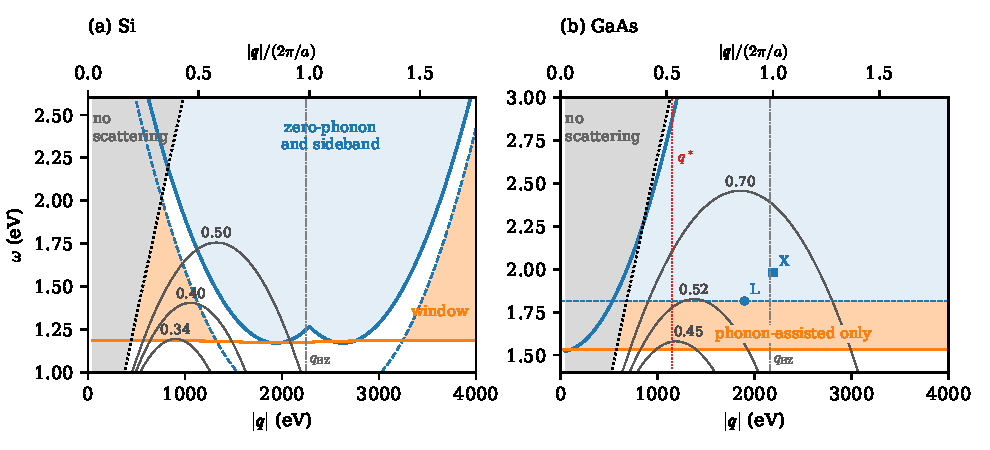
\includegraphics[width=\linewidth]{figures/ch17/fig17_4.pdf}
  \caption{Where the Migdal--phonon-assisted interference enters, in the plane of momentum transfer and energy deposited by scattering. (a)~Silicon. Thick blue: zero-phonon edge of the parabolic valleys along [100], $E_{\mathrm{min}} = \Eg + (q - K)^2/2M_{\mathrm{eh}}$ with $\Eg = \SI{1.17}{eV}$, $M_{\mathrm{eh}} = 1.193\,m_e$, $K = k_{\mathrm{c}} = 0.85\,(2\pi/a)$ and its images under $(2,0,0)\,2\pi/a$, a model that lies \SI{0.13}{eV} above the computed bands at \SI{1}{keV}. Dashed blue: the same lowered by the off-shell margin of the window, $\delta_w = \SI{0.3}{eV}$ (\cref{sec:8.6}). Orange line: the phonon-assisted threshold $\Eg + \omega_{\mathrm{TA}}(k_{\mathrm{c}} - q)$. Orange: the window, where the phonon-dressed sector is the only electronic final state and the cross term of \cref{eq:17.4-Sek} is a fraction of the whole electronic rate. White strip: the edge shell within $\delta_w$ of the zero-phonon edge, where only the sum of the two electronic sectors is defined. Light blue: zero-phonon pairs, with the phonon-dressed sector and its cross term a correction. (b)~GaAs: edge of the $\mathrm{\Gamma}$ pair with the [111] heavy hole ($\Eg = \SI{1.52}{eV}$, $M_{\mathrm{eh}} = 0.960\,m_e$), the L and X valleys at 1.815 and \SI{1.981}{eV} (points at $|\mathrm{\Gamma L}|$ and $|\mathrm{\Gamma X}|$), and the phonon-assisted threshold with the upper value \SI{10.5}{meV} of the transverse acoustic branch. Orange: below both the $\mathrm{\Gamma}$ edge and the L energy, phonon-assisted pairs only; the L valleys reach the line $\omega = \SI{1.815}{eV}$ near $|\mathrm{\Gamma L}|$ only. Red dotted: $q^* = \SI{1.15}{keV}$ of the GaAs window. Both panels: the largest deposit $qv_{\mathrm{max}} - q^2/2\mchi$ for the masses marked in MeV (gray), the envelope $qv_{\mathrm{max}}$ (dotted; gray region unreachable by scattering), and $q_{\mathrm{BZ}}$, the radius of the sphere with the volume of the zone (dash-dotted). Top axes: $q$ in units of $2\pi/a$; \cref{eq:17.4-lock} holds for $q \ll q_{\mathrm{BZ}}$.}
  \label{fig:17-interference}
\end{figure}

\Cref{fig:17-interference} places the cross term in the plane of $q$ and $\omega$. It exists wherever a pair with one phonon is kinematically allowed, above the phonon-assisted threshold, but it changes an observable rate by more than a correction to a correction in the window alone. There the phonon-dressed sector is the whole electronic rate of silicon between 0.3374 and \SI{0.405}{MeV} (\cref{tab:13-window}), and of GaAs from \SI{0.433}{MeV} to the opening of the L valleys at 0.52 to \SI{0.56}{MeV} (\cref{sec:13.1}).

\begin{workedexample}{The cross terms of a heavy dark photon in GaAs}\label{we:17-gaas-interference}
Take a dark photon with a heavy mediator, $\FDM = 1$, so that $\tilde V_e = \tilde V$ and $\tilde V_\kappa = -Z_\kappa\tilde V$ with $\tilde V$ independent of $q$, scattering in GaAs at $T = 0$. In the window it makes pairs only with a phonon, at momentum transfers near $q^* = \SI{1.15}{keV}$, 0.52 of $2\pi/a = \SI{2.193}{keV}$ (\cref{fig:17-interference}b).

\emph{Electron-following cell.} With $|Z^*| = 2.11$ (\cref{sec:5.5}), a gallium nucleus carries $Z = 31$ and its cloud $F^{\mathrm{fol}} = 28.89$ at long wavelength; an arsenic nucleus $Z = 33$ and $F^{\mathrm{fol}} = 35.11$. The separate terms are $961 + 834.6$ and $1089 + 1232.7$, the cross terms $-1791.2$ and $-2317.3$, and each total is $Z^{*2} = 4.452$: the cross term removes \SI{99.75}{\percent} and \SI{99.81}{\percent} of the two separate terms. The optical phonons that the dark photon makes are those of \cref{sec:11.2}. Without the cross cell their rate would be $(Z^2 + (F^{\mathrm{fol}})^2)/Z^{*2} = 403$ times (gallium) and 521 times (arsenic) larger, and the bare nuclear charges alone would give 216 and 245 times more, before the screening by $\varepsilon_\infty$ that both cases share.

\emph{Zero-phonon cell.} Above the opening of the L valleys the zero-phonon rate gains $2m_e\bar z$ from the ionic correction. The two values of $Z/M$, 0.4446 per u for gallium and 0.4405 per u for arsenic, differ by \SI{0.9}{\percent}. With $m_e = 5.486\times10^{-4}$\,u the cross cell is $4.88\times10^{-4}$ for weight on gallium alone and $4.83\times10^{-4}$ for weight on arsenic alone, and lies between the two for any positive weights. The zero-phonon Migdal cell is $(m_e\bar z)^2 = 5.9\times10^{-8}$.

\emph{Phonon-dressed cell.} In the window the whole electronic rate is phonon-assisted, and at leading order in $q$, \cref{eq:17.4-rate} with the mass-weighted mean gives it the same fraction, $4.8$ to $4.9\times10^{-4}$, and the one-phonon Migdal rate $5.9\times10^{-8}$ of it. Since $\mathfrak{D}$ has no $q$ dependence for a heavy mediator, the fraction is the same at every momentum transfer at this order, and the integrated rate carries it unchanged. At $q^*$, however, $q/(2\pi/a) = 0.52$, and the remainder of \cref{eq:17.4-lock} is not small. The cross term is of order $5\times10^{-4}$ of the phonon-assisted rate, with an uncertainty of order one in that fraction.

\emph{Screening.} The dark photon couples to the total charge, and both rows share the screening $1/\varepsilon$ of the total-charge row (\cref{sec:8.4}), which cancels from every fraction above.

\emph{Verdict.} The phonon-assisted rate of the silicon window is an estimate known to a factor of ten (\cref{tab:13-window}), and the GaAs window is known through its edges (\cref{sec:13.1}). The two electronic cross terms lie more than three orders of magnitude below such uncertainties. For a dark photon in GaAs the electron-following cell is the one that matters, and it decides the phonon rate.
\end{workedexample}

At small $q$ the nuclear amplitude in the electronic sectors is $(m_e/M_\kappa)\tilde V_{\mathrm{nuc}}/\tilde V_e$ times the electron amplitude. The cross term competes with the electron term when the coupling to a nucleus exceeds that to an electron by $M_\kappa/m_e = 5.1\times10^4$ in silicon, or, per nucleon, by $m_{\mathrm{u}}/m_e = 1823$. A scalar mixed with the Higgs boson, whose couplings follow the masses up to the nucleon matrix element, comes close to this; a $B - L$ vector, with couplings of equal size per nucleon and per electron, is far from it. For such a mediator a Migdal rate and an electron-recoil rate computed separately and added miss the true rate by the full cross term.
